\section{Semantics | Semantic Parsing}
\subsection*{Description}
\emph{Task} --- Assign semantic structure, i.e. logical form, to a sentence

{\color{lightgray}\hrule height 0.001mm}

\emph{Description} ---
\begin{itemize}
    \item \emph{Principle of compositionality}:
    \begin{itemize}
        \item The meaning of a complex expression is a function of the meanings of that expression's constituent parts
        \item Thus, we can syntactically parse a sentence and then construct the semantic representation bottom-up
    \end{itemize}
    \item Applying the principle of compositionality:
    \begin{itemize}
        \item Syntactic rule, e.g. $\textrm{S} \to \textrm{NP VP}$
        \item Induces semantic rule, e.g. $\textrm{s.sem} \to \textrm{VP.sem} (\textrm{NP.sem})$: Semantic representation of sentence $s$ is a function of the semantic representation of the verb phrase, applied to the semantic representation of the noun phrase
    \end{itemize}
\end{itemize}

{\color{black}\hrule height 0.001mm}

\subsection*{Lambda Calculus}
\emph{Basics} ---
\begin{itemize}
    \item Basic components:
    \begin{itemize}
        \item Logical constants: Represent objects (e.g. Boston) and relations (e.g. likes)
        \item Variables:
        \begin{itemize}
            \item Undetermined logical constants
            \item Objects are represented in lowercase as $x, y, z, \dots$ and are input to $\lambda x.f(x)$
            \item Relations are represented in uppercase as $P, Q, R, \dots$ and are input to $\lambda P.P(\dots)$
            \begin{itemize}
                \item \emph{Free variables}: Do not occur in the scope of any abstraction that holds its name
                \item Otherwise, \emph{bound variables}: Bound by the abstraction with the smallest scope
                \item E.g. $((\textcolor{orange}{\lambda x[}.\textcolor{red}{\lambda y[}.(\textcolor{orange}{x} ((\textcolor{blue}{\lambda x.[x]} \textcolor{orange}{x}) \textcolor{red}{y}))\textcolor{red}{]}\textcolor{orange}{]} \textcolor{green}{\lambda x.[x]}) z)$ where
                \begin{itemize}
                    \item $z$ is unbound
                    \item Other variables are bound by same-colored abstractions
                    \item Scopes of abstractions are indicated by square brackets
                \end{itemize}
            \end{itemize}
        \end{itemize}
        \item Every relation has an \emph{arity} that determines the number of objects it relates (e.g. $P(x, y)$ has arity $2$)
        \item \emph{Literals}: Formed by applying relations to objects (e.g. likes(Alex, y), $P(x, y)$)
        \item Logical connectives and quantifiers: $\exists, \forall, \neg, \land, \lor$
    \end{itemize}
    \item New terms can be constructed using $2$ recursive rules:
    \begin{itemize}
        \item 1) Abstraction:
        \begin{itemize}
            \item If $M$ is a term, $N$ is a term, and $x$ is a variable:
            \begin{itemize}
                \item $\lambda x$ is an \emph{abstraction}
                \item $\lambda x.M$ is a function with input $x$ and \emph{scope of abstraction} $M$. It replaces every free occurrence of $x$ in $M$ with whatever the function is applied to (e.g. $N$)
                \item $\lambda x.M N$ is a function applied to $N$
                \item We denote the output of $\lambda x.M N$ as $M[x := N]$
                \item Note: 
                \begin{itemize}
                    \item In the output of $\lambda x.M N$, only $M[x := N]$ remains, and $\lambda x.$ and $N$ disappear
                    \item In $M[x := N]$ for relations $P(x)$, the relation $P$ is exchanged, but the arguments $x$ are left untouched
                    \item Work from outside in
                    \item Determine what is applied to what based on what is the argument in the CCG expression $X \mid Y$ (e.g. if $Y$ is the argument in $X / Y$, then the lambda expression is applied to $Y$: $\lambda x.M Y$)
                \end{itemize}
            \end{itemize}
            \item When forming abstraction (i.e. $M \to \lambda x.M$), already bound occurrences of $x$ in $M$ remain bound by inner $\lambda$, free occurrences of $x$ become bound by outer $\lambda$
        \end{itemize}
        \item 2) Application: If $M$ and $N$ are terms, $(MN)$ is a term
        \begin{itemize}
            \item When forming application (i.e. $M \to MN$), already bound occurrences of $x$ in $M$ remain bound by inner $\lambda$, free occurrences of $x$ remain free
        \end{itemize}
    \end{itemize}
\end{itemize}

{\color{lightgray}\hrule height 0.001mm}

\emph{Alpha conversion} ---
\begin{itemize}
    \item Process of renaming a variable in a lambda term 
    \item We can rename a variable in an abstraction together with all its occurrences in the scope of the abstraction
    \item If the renamed variable remains bound to the same abstraction and the remaining variables remain free resp. bound as before, the renaming is valid
    \item E.g. 
    $\lambda x.\lambda y.(x((\lambda x. x x) y )) \to \lambda z. \lambda y. (z((\lambda x. x z) y))$ is valid\\
    $\lambda x.(xy) \to \lambda y.(yy)$ is not valid, since $y$ was free before and is now bound
\end{itemize}

{\color{lightgray}\hrule height 0.001mm}

\emph{Beta reduction} ---
\begin{itemize}
    \item Process of applying one lambda term to another: $(\lambda x.M)N$
    \item We can apply one lambda term to another if the free variables in $N$ remain free in $M[x := N]$
    \item If this is not the case, first apply alpha-conversion to $M$
    \item Termination issue: Repeatedly applying beta reductions may not terminate
    \item E.g. $\lambda y.(z((\lambda x.\textcolor{blue}{\mathbf{x}}\textcolor{orange}{z})y)) \to \lambda y.(z(\textcolor{red}{z}y))$\\
    $(\lambda x.\textcolor{blue}{\lambda y.(\mathbf{x}((\lambda x.x\mathbf{x})y))}\textcolor{orange}{z}) \to \lambda y.(\textcolor{red}{z}((\lambda x.x\textcolor{red}{z})y))$
    where
    \begin{itemize}
        \item $\textcolor{blue}{blue}$ corresponds to $M$
        \item $\textcolor{orange}{orange}$ corresponds to $N$
        \item $\textcolor{red}{red}$ corresponds to $M[x := N]$
        \item $\boldsymbol{bold}$ corresponds to free variables in $M$
    \end{itemize}
\end{itemize}

{\color{lightgray}\hrule height 0.001mm}

\emph{Equivalence} --- Two lambda terms are equivalent if they can be obtained from each other via a series of $\alpha$- and $\beta$-conversions

{\color{black}\hrule height 0.001mm}

\subsection*{Linear Indexed Grammar resp. Combinatory Categorial Grammars (CCG)}
\emph{Features} --- 
\begin{itemize}
    \item LIG, CCG: Mildly context sensitive
    \item LIG, CCG: Support languages with complex or free word order (e.g. cross-serial dependencies, long-distance dependencies, coordination)
    \item CCG: \emph{Compositionality}: Semantic representation of a sentence is built in tandem with its syntactic derivation
    \item The latter two are advantages over CFGs
\end{itemize}

{\color{lightgray}\hrule height 0.001mm}

\emph{Linear Indexed Grammar $\langle \mathcal{N}, S, \mathcal{I}, \Sigma, \mathcal{R} \rangle$} --- 
\begin{itemize}
    \item $\mathcal{N}$: Set of non-terminals $N_1, N_2, N_3, \dots$
    \item $S$: Start non-terminal
    \item $\mathcal{I}$: Finite set of indices $f, g, h, \dots$
    \item $\Sigma$: Alphabet of terminals $a_1, a_2, a_3, \dots$
    \item $\mathcal{R}$: Set of production rules of the following forms:
    \begin{enumerate}
        \item $N[\sigma] \to \alpha M[\sigma]\beta$
        \item $N[\sigma] \to \alpha M[f\sigma]\beta$
        \item $N[f\sigma] \to \alpha M[\sigma]\beta$
    \end{enumerate}
    \begin{itemize}
        \item Where
        \begin{itemize}
            \item $N$ and $M$ are non-terminals
            \item $\alpha$ and $\beta$ are sequences of terminals and non-terminals
            \item $\sigma$ is associated with the non-terminal on the LHS and passed to exactly one non-terminal on RHS
            \item For a stack, base symbol $\sigma$ is usually combined with a marker $f$, where markers encode a count and can be popped from (rule 3) or pushed to (rule 2) the stack
        \end{itemize}
    \end{itemize}
    \item Can generate languages, which cannot be generated by CFG. E.g. language $\{a^n b^n c^n d^n : n \geq 0\}$ via rules:
    \begin{itemize}
        \item $S[\sigma] \to aS[\sigma f]d$
        \item $S[\sigma] \to T[\sigma]$
        \item $T[\sigma f] \to bT[\sigma]c$
        \item $T[\varepsilon] \to \varepsilon$
    \end{itemize} 
\end{itemize}

{\color{lightgray}\hrule height 0.001mm}

\emph{Combinatory Categorial Grammar $\langle \mathcal{V}_T, \mathcal{V}_N, S, f, \mathcal{R} \rangle$} --- 
\begin{itemize}
    \item $\mathcal{V}_N$: \emph{Atomic categories}: Set of non-terminals
    \item $S$: Start non-terminal
    \item $\mathcal{V}_T$: Set of terminals
    \item $\mathcal{R}$: Set of production rules 
    \item $f: \mathcal{V}_T \to \mathcal{C}(\mathcal{V}_N)$: \emph{Lexicon}: Function that maps elements of $\mathcal{V}_T \cup \{\varepsilon\}$ to finite subsets of $\mathcal{C}(\mathcal{V}_N)$ 
    \item $\mathcal{C}(\mathcal{V}_N)$: Set of \emph{categories}, including \emph{atomic} and \emph{complex} categories
\end{itemize}
Deep-dive on categories, rules, and lexicon:
\begin{itemize}
    \item Categories: 
    \begin{itemize}
        \item \emph{Atomic categories}: 
        \begin{itemize}
            \item Complete constituents
            \item Terminals
        \end{itemize}
        \item \emph{Complex categories}:
        \begin{itemize}
            \item Incomplete constituents
            \item Built recursively from atomic categories via operators
            \item Function that specifies the type of result and type and direction of its arguments
            with pattern: $X \mid Y \quad Y \to X$, where 
            \begin{itemize}
                \item $X \mid Y$ is function, with $\mid$ being an operator, $Y$ being argument, and $X$ being output
                \item Applying function to $Y$ yields $X$
            \end{itemize}
            \item \emph{Operators}:
            \begin{itemize}
                \item Backward slash: $X \backslash Y$: "Give me argument $Y$ to my left, and I return an $X$"
                \item Forward slash: $X / Y$: "Give me argument $Y$ to my right, and I return an $X$"
                \item Operators need to be read from outside in, e.g. $(\textrm{S} \backslash \textrm{NP}) / \textrm{NP}$: Needs $\textrm{NP}$ to its right, then needs $\textrm{NP}$ to its left, then produces sentence $\textrm{S}$
            \end{itemize}
            \item Complex categories have an \emph{arity} that determines the number of arguments it has (e.g. $X / Y \backslash Z$ has arity $2$)
        \end{itemize}
        \item Every category can be written in the form $X = A \mid_m X_m \dots \mid_1 X_1$ where
        \begin{itemize}
            \item $A$: Atomic category, output of $X$
            \item $X_1, \dots, X_m$: Arbitrary categories, arguments of $X$
            \item $\mid$ = $/$ or $\backslash$, whether $X$ expects argument on right or left side
            \item $m$ = Arity of $X$, $\geq 0$
        \end{itemize}
        \item Set of categories $\mathcal{C}(\mathcal{V}_N)$ is the smallest set such that:
        \begin{itemize}
            \item If $C \in \mathcal{V}_N$, then $C \in \mathcal{C}(\mathcal{V}_N)$
            \item If $C_1, C_2 \in \mathcal{V}_N$, then $(C_1 / C_2) \in \mathcal{C}(\mathcal{V}_N)$ and $(C_1 \backslash C_2) \in \mathcal{C}(\mathcal{V}_N)$
        \end{itemize}
    \end{itemize}
    \item Rules:
    \begin{itemize}
        \item Specify how categories can be combined into other categories
        \item \emph{Function application}:
        \begin{itemize}
            \item \emph{Forward application} $(>)$: If a category expects an argument to the right of $(X / Y)$ and argument $Y$ is available, they combine to form $X$: $X / Y \quad Y \to X$
            \item \emph{Backward application} $(<)$: If a category expects an argument to the left of $(X \backslash Y)$ and argument $Y$ is available, they combine to form $X$: $Y \quad X \backslash Y\to X$
            \item Have \emph{primary input} (function part in rule) and \emph{secondary input} (argument part in rule) 
            \item \emph{AB grammar resp. basic categorical grammar resp. pure categorical grammar}: CCGs that only have application rules, have power of CFG:
            $
            A \to a \text{ in CCG} \equiv A \to a \text{ in CFG}
            $\\
            $
            A \to (A / C) C \text{ in CCG} \equiv A \to BC \text{ in CFG}
            $
        \end{itemize}
        \item \emph{Function composition}:
        \begin{itemize}
            \item Two functions combine to form a single function: $f, g \to f \circ g$
            \item \emph{Forward composition} $((B_>$: $(X / Y) \quad (Y / Z) \to (X / Z)$
            \item \emph{Backward composition} $((B_<)$: $(Y \backslash Z) \quad (X \backslash Y) \to (X \backslash Z)$
        \end{itemize}
        \item \emph{Higher-order rules}:
        \begin{itemize}
            \item \emph{Forward} $(>^n)$:
            $
            X/Y \ Y \mid_n Y_n ... \mid_1 Y_1 \to X \mid_n Y_n ... \mid_1 Y_1 
            $
            \item \emph{Backward} $(<^n)$:
            $
            Y \mid_n Y_n ... \mid_1 Y_1 \ X \backslash Y \to X \mid_n Y_n ... \mid_1 Y_1 
            $
            \item $n$ is the \emph{degree} of the rule
            \item If $n=0$, corresponds to application rule
        \end{itemize}
        \item \emph{Type raising}:
        \begin{itemize}
            \item Turn an atomic category into a complex category so it can participate in higher-order functions
            \item \emph{Forward type raising} $(T_>)$:
            $
            X \to T / (T \backslash X)
            $
            \item \emph{Backward type raising} $(T_<)$:
            $
            X \to T \backslash (T / X)
            $
            \item E.g.
            Intransitive $\textrm{S} \backslash \textrm{NP}$ (e.g. walked)\\
            Transitive $(\textrm{S} \backslash \textrm{NP}) / \textrm{NP}$ (e.g. respected)\\
            Ditransitive $((\textrm{S} \backslash \textrm{NP}) / \textrm{NP}) / \textrm{NP}$ (e.g. gave)
        \end{itemize}
        \item Rule instance is obtained by substituting $X, Y, Z, \dots$ by concrete categories, e.g. $\textrm{S, NP, VP}$, etc.
        \item CCGs have finite set of rules ($2^{|\mathcal{V}_N|}$ forward, $2^{|\mathcal{V}_N|}$ backward rules) but infinitely many rule instances
    \end{itemize}
    \item Lexicon: Associates terminals with categories, encodes the structure (vs. CFG, where rules encodes the structure)
    \begin{itemize}
        \item E.g. entry in lexicon for atomic category: $\textrm{Harry} := NP$
        \item E.g. entry in lexicon for complex category: $\textrm{walks} := (S \backslash NP)$
    \end{itemize}
\end{itemize}
CCG parsing:
\begin{itemize}
    \item General rule of inference:
    $
    \frac{A_1 \quad \dots \quad A_k}{B}
    $
    where $B$ is a consequence of $A_1, \dots, A_k$
    \item \emph{Derivation trees}:
    \begin{itemize}
        \item Consist of unary and binary branches
        \item \emph{Unary branches}: Rules for atomic categories
        \item \emph{Binary branches}: Rules for complex categories
    \end{itemize}
\end{itemize}
CCG parsing | CKY-style parsing algorithm:
\begin{itemize}
    \item Let $w$ be the sentence of length $n$ to be parsed, $w_i$ be a token in the sentence, and $w[i, j]$ be the substring from $w_{i+1} \dots w_j$, and $w_{ii} = \varepsilon$
    \item Aim: Construct item $[S, 0, n]$, i.e. we can construct sentence based on words between positions $1$ and $n$
    \item Derivation tree leading to this outcome has internal nodes $[X, i, j]$ i.e. we can construct category based on words between positions $i+1$ and $j$
    \item \emph{Axioms}: $[X, i, i+1]$ where $w_{i+1} = X$ is a lexicon entry
    \item \emph{Inference rules}:
    \begin{itemize}
        \item 
        $
        \frac{[X / Y, i, j] \quad [Y \beta, j, k]}{[X \beta, i, k]} \quad X / Y \quad Y \beta \to X \beta
        $\\
        resp.\\
        $
        \frac{[Y \beta, i, j] \quad [X \backslash Y, j, k]}{[X \beta, i, k]} \quad Y \beta \quad X \backslash Y \to X \beta
        $
    \end{itemize}
    \item Challenge: With the composition rule, we can grow the arity of the primary input categories and get exponentially many primary input categories
    \item Solution: Restrict the arity of the categories
\end{itemize}
CCG parsing | Polynomial time algorithm:
\begin{itemize}
    \item Arity of categories is bounded by \emph{grammar constant} $C_g$:
    $[X, i, j]$ where $\textrm{ar}(X) \leq C_g$
    \item Challenge: Categories with arity $> C_g$ can no longer be derived
    \item Solution:
    \begin{itemize}
        \item Introduce new rules that decompose longer derivations into smaller pieces
        \item \emph{Derivation context} $c$:
        \begin{itemize}
            \item Configuration in derivation, where there are two subtrees $t'$ and $c$, which together form subtree $t$
            \item $t$ parses the segment $w_{[i,j]}$ in the sentence, $t'$ parses $w_{[i,i']}$ thereby deriving the function $\cdots X \mid Y$, and $c$ parses $w_{[j',j]}$ thereby deriving the corresponding argument $Y \cdots$
            \item $t'$ and $c$ combine to form $\cdots X \cdots$ which represents the entire derivation $t$ for $w_{[i,j]}$
            \item None of the combinatory rules used in $c$ touches $X$, i.e. $c$ only operates on $Y$
            \item For this reason, $c$ is a derivation context and can be re-used across multiple derivations for $X$ 
        \end{itemize}
        \item New inference rules:
        \begin{itemize}
            \item Next to normal inference rules above
            
            \item 1) If the composition of two categories ($X \mid Y \quad Y\beta$) would result in a category with arity $\text{ar}(X \beta) > C_g$:\\
            Context item is derived:
            $
            \frac{[X / Y, i, j] \quad [Y \beta, j, k]}{[/ Y, \beta, i, i, j, k]}
            $\\
            resp.\\
            $
            \frac{[Y \beta, i, j] \quad [X \backslash Y, j, k]}{[\backslash Y, \beta, i, i, j, k]}
            $ ??? \\
            where $\beta$ are all non-terminals and edge operators, except for $Y$

            \item 2.1) If the further composition of a context item with another category ($X \mid Y \quad Y \beta$) would result in a category with arity $\text{ar}(X \beta) \leq C_g$:\\ 
            Context item can be recombined with the original derivation:
            $
            \frac{[X / Y, i', j'] \quad [/ Y, \beta, i, i', j', j]}{[X \beta, i, j]}
            $\\ 
            resp.\\
            $
            \frac{[\backslash Y, \beta, i, i', j', j] \quad [X \backslash Y, i', j']}{[X \beta, i, j]}
            $ ?
            
            \item 2.2.1) If the further composition of a context item with another category ($\beta \mid Z \quad Z_\gamma$) would result in a category with arity $\text{ar}(Y \beta_\gamma) \leq C_g$:\\ 
            Context item can be extended normally, similar to derivation trees:
            $
            \frac{[\mid Y, \beta / Z, i, i', j', j] \quad [Z_\gamma, j, k]}{[\mid Y, \beta_\gamma, i, i', j', k]}
            $\\
            resp.\\
            $
            \frac{[Z_\gamma, i, j] \quad [\mid Y, \beta \backslash Z, j, j', k', k]}{[\mid Y, \beta_\gamma, i, j', k', k]} 
            $ ? \\
            where $\beta_\gamma$ refers to $\beta$ without $/ Z$ (can be $\varepsilon$)

            \item 2.2.2) If the further composition of a context item with another category would result in a category with arity $\text{ar}(Y \beta_\gamma) > C_g$:\\
            A new context is derived from the previous context:
            $
            \frac{[\mid Y, \beta / Z, i, i', j', j] \quad [Z_\gamma, j, k]}{[/ Z, \gamma, i, i, j, k]}
            $\\
            resp.\\
            $
            \frac{[Z_\gamma, i,j] \quad [\mid Y, \beta \backslash Z, j, j', k', k]}{[\backslash Z, \gamma, i, i, j, k]}
            $ ???
            
            \item 3.1) When the arity is small enough, the new context item can be recombined with the previous context:
            $
            \frac{[\mid Y, \beta / Z, i'', i', j', j''] \quad [/ Z, \varepsilon, i, i'', j'', j]}{[\mid Y, \beta, i, i', j', j]}
            $\\
            resp.\\
            $
            \frac{[\backslash Z, \varepsilon, i'', i', j', j''] \quad [\mid Y, \beta \backslash Z, i, i'', j'', j]}{[\mid Y, \beta, i, i', j', j]}
            $ ???
        \end{itemize}
    \end{itemize}
    \item Grammar constant $C_g$ is at least as large as maximal $Y$ (determined by largest arity $a$ in lexicon) and $\beta$ (determined by the maximum degree $n$ of composition rules), since we need to restrict the size of $Y \beta$
    \item Together: $C_g \geq \max \{ \ell, a + n \}$
\end{itemize}
CCG combine syntactic and semantic information when paired with lambda calculus:
\begin{itemize}
    \item E.g.\\
    Mary $:= \textrm{NP} : \textrm{MARY}(x)$\\
    likes $:= (\textrm{S} \backslash \textrm{NP}) / \textrm{NP} : \lambda x.\ \lambda y.\ \textrm{likes}(x, y)$\\
    natural language $:=$ syntax $:$ semantics
    \item If we parse a sentence syntactically, we can derive semantics bottom-up in the same order, working from smallest constituents to highest constituents
\end{itemize}

{\color{black}\hrule height 0.001mm}

\subsection*{SK-Calculus resp. Combinatory Logic}
\begin{itemize}
    \item Alternative to lambda calculus
    \item Basic terms:
    \begin{itemize}
        \item \emph{Variables}: $x, y, z, \dots$
        \item \emph{Primitive functions resp. combinators}: 
        \begin{itemize}
            \item $S$ \emph{combinator}: $Sxyz = (xz(yz)) = ((xz)(yz)$
            \item $K$ \emph{combinator}: Constant function: $Kxy = ((Kx)y) = x$
            \item $I$ \emph{combinator}: Identity function: $Ix = x$
            \item $B$ \emph{combinator}: Composition function: $Bxyz = (x(yz))$
            \item $C$ \emph{combinator}: $Cxyz = ((xz)y)$
            \item $T$ \emph{combinator}: Type-raising function: $Txy = yx$
        \end{itemize}
    \end{itemize}
    \item Terms are recursively constructed via application: If $M$ and $N$ are terms, $(MN)$ is a term
    \item Parentheses are left-associative, e.g. $(Kxyz) = (((Kx)y)z)$
    \item \emph{SK calculus}: Only leverages $S$ and $K$ operator
    \begin{itemize}
        \item $SKK$ and $I$ are extensionally equivalent: $S(KK)x = SKKx = K x(K x) = x$
        \item Therefore, the $SK$ basis is complete, and we don't need $I$ operator
    \end{itemize}
\end{itemize}

{\color{black}\hrule height 0.001mm}

\subsection*{Transforming Lambda Calculus into SK-Calculus}
Apply recursively defined transformation $T$:
\begin{enumerate}
    \item $T(x) = x$ for every variable $x$
    \item $T[(E_1E_2)] = (T[E_1]T[E_2])$ for all lambda terms $E_1$, $E_2$
    \item $T[\lambda x.E] = (KT[E])$ for every lambda term $E$ where $x$ is either bound or absent within the term
    \item $T[\lambda x.x] =  (SKK) = I$
    \item $T[\lambda x.\lambda y.E] = T[\lambda x.T[\lambda y.E]]$ for every lambda term $E$ where $x$ is free within the term
    \item $T[\lambda x.(E_1E_2)] = (ST[\lambda x.E_1]T[\lambda x.E_2])$ for all lambda terms $E_1, E_2$ where $x$ is free within at least one of the two terms
\end{enumerate}

\begin{multicols}{2}
\textit{1) Semantic and syntactic parse}\\
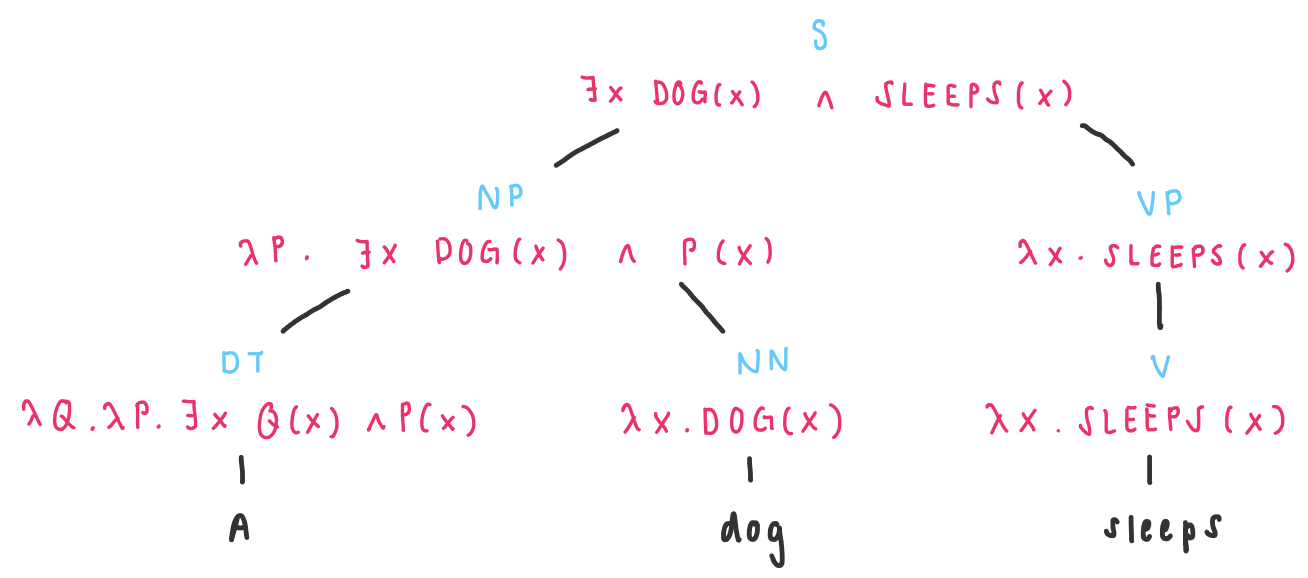
\includegraphics[height=10mm]{inhalt/images/NLP/06_semantic_parsing_1.png}
\\\\
\textit{2) Derivation context}\\
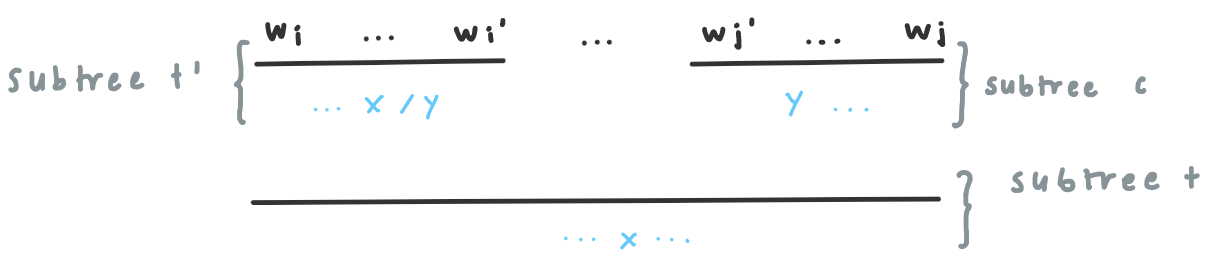
\includegraphics[height=10mm]{inhalt/images/NLP/06_semantic_parsing_2.png}
\\\\
\textit{3) CCG parsing: Derivation trees}\\
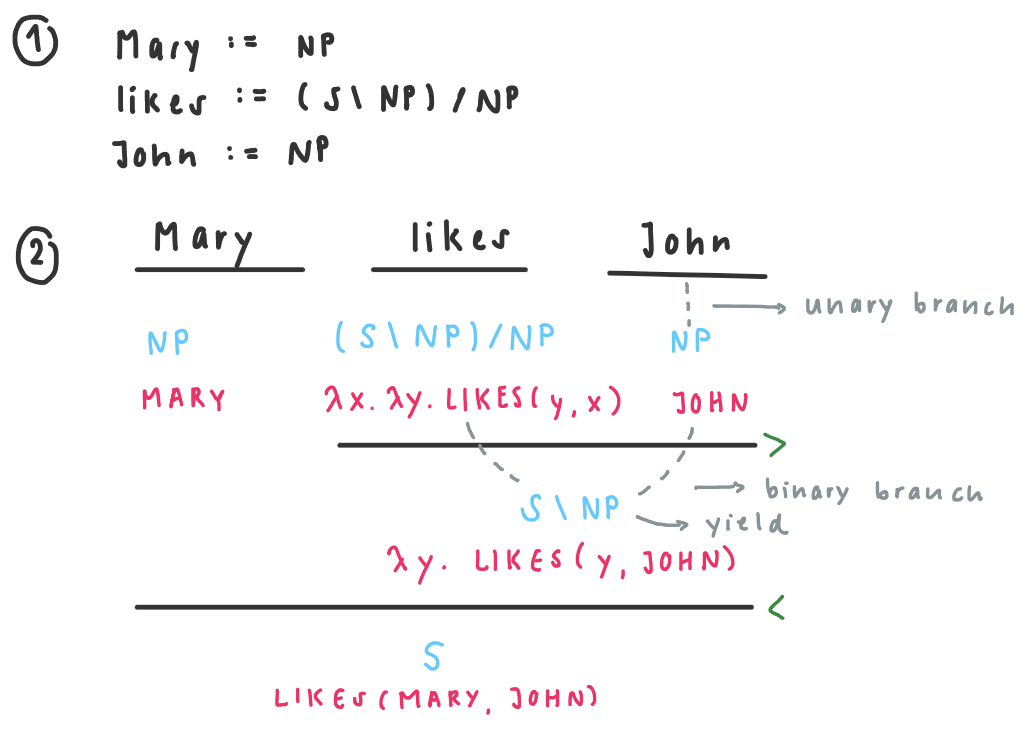
\includegraphics[height=25mm]{inhalt/images/NLP/06_semantic_parsing_3.png}
\\\\
\end{multicols}
\textit{4) Linear indexed grammar: Example for language, which can be generated by LIG but not CFG}\\
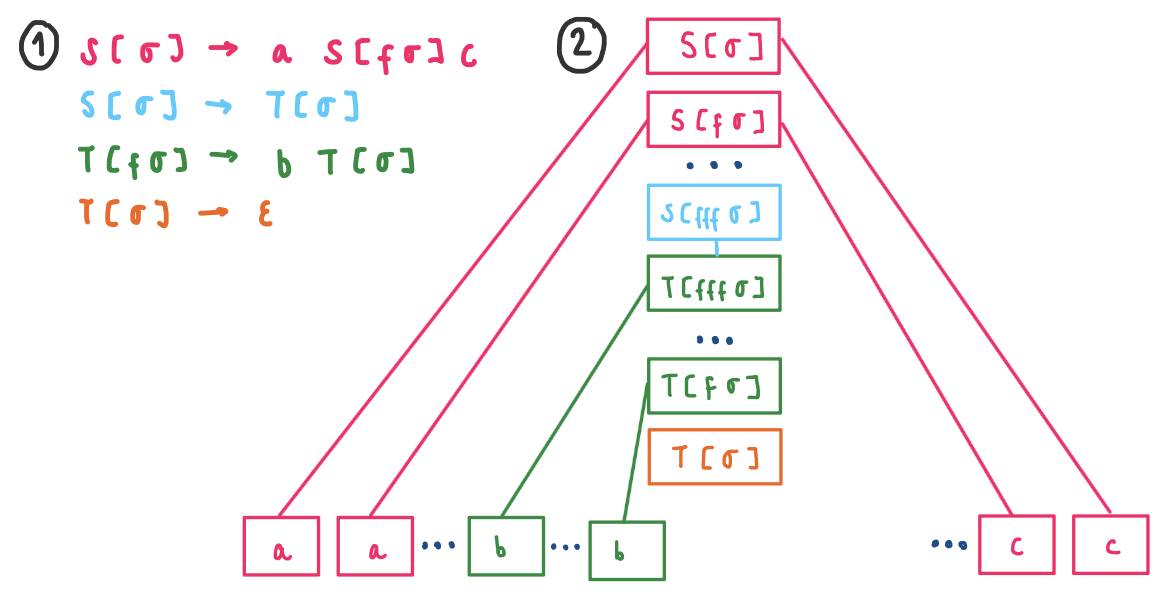
\includegraphics[height=25mm]{inhalt/images/NLP/06_semantic_parsing_4.png}
\\\\
\textit{5) Polynomial time algorithm}\\
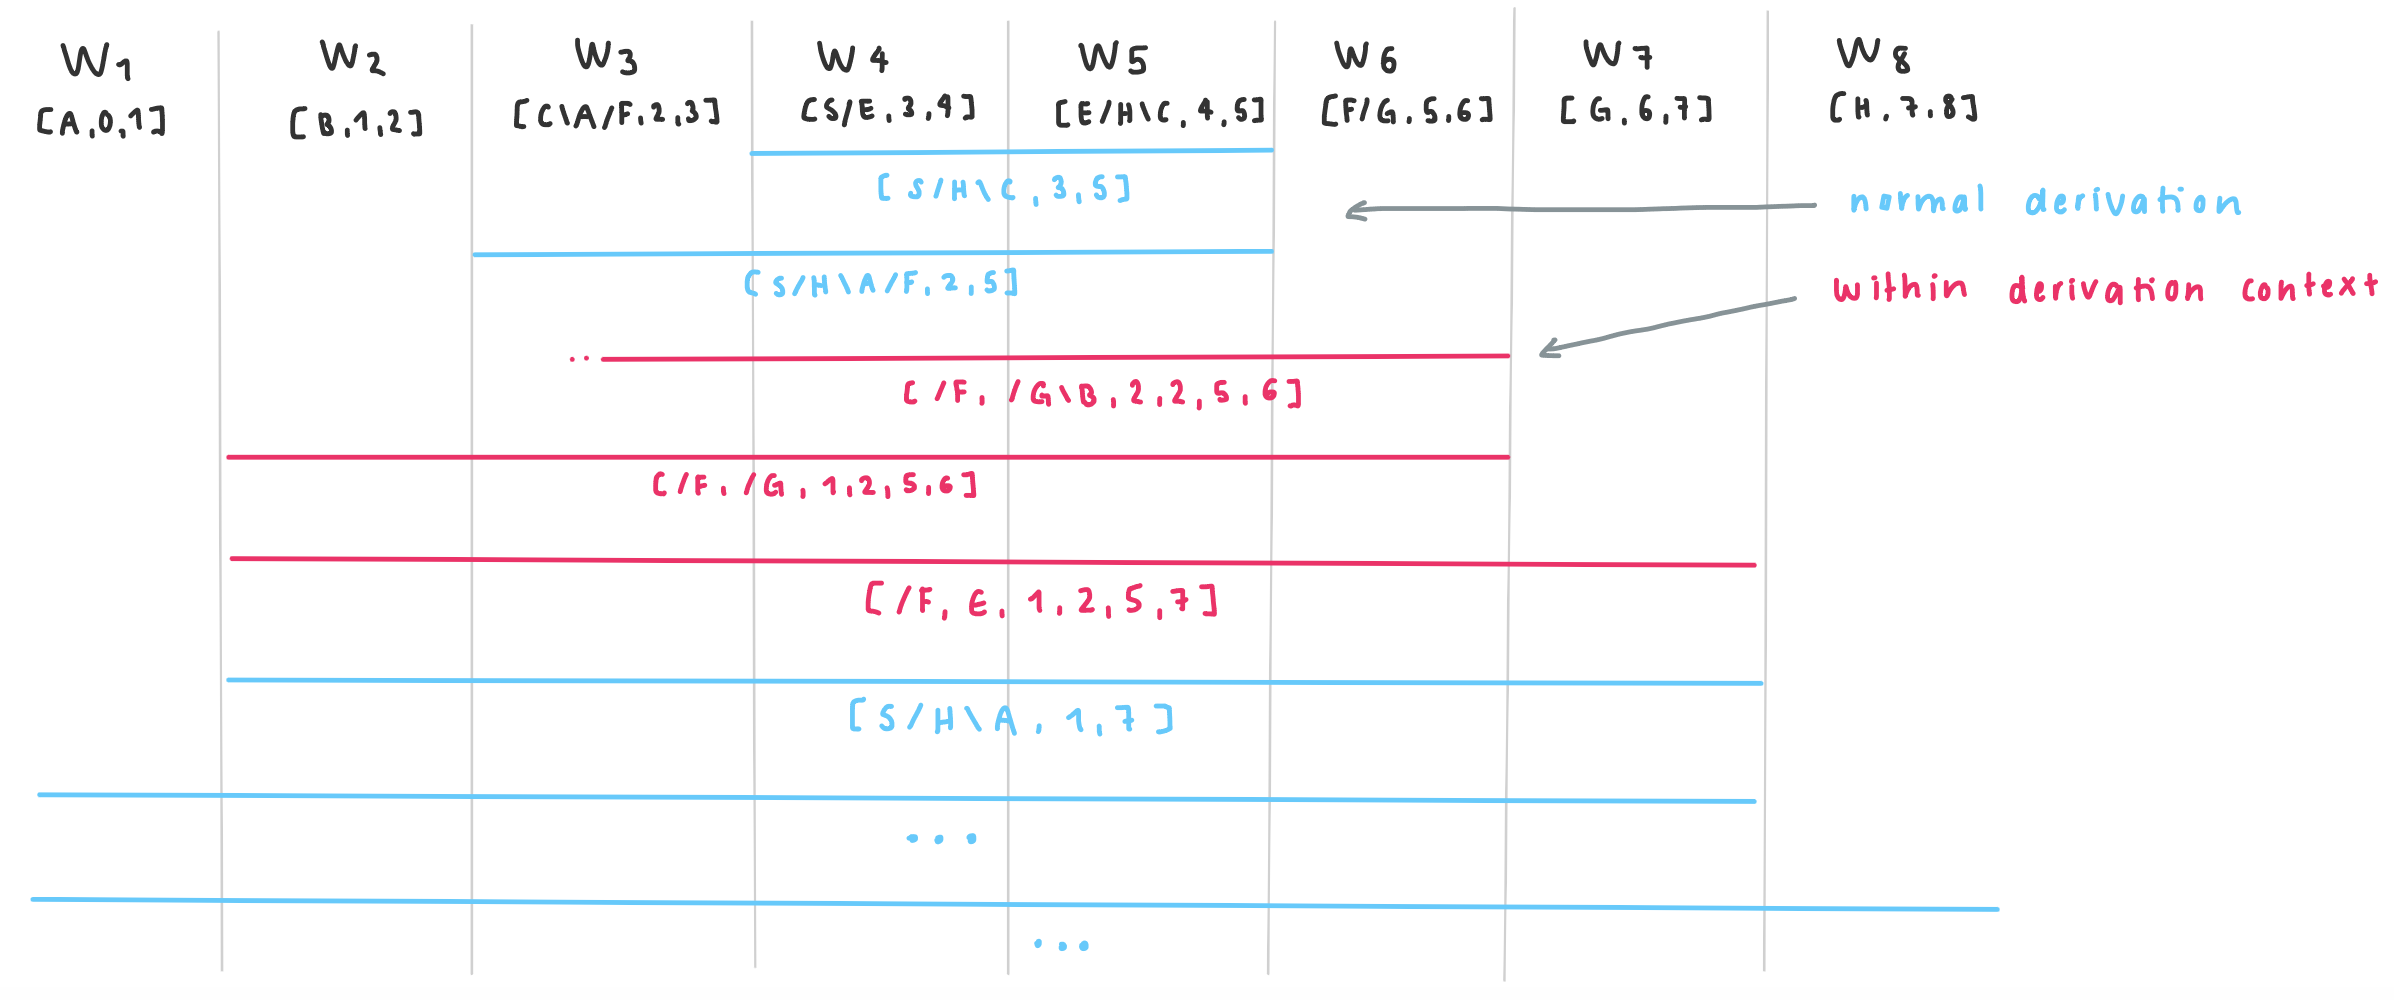
\includegraphics[height=25mm]{inhalt/images/NLP/06_semantic_parsing_5.png}
\\\\